\documentclass[10pt,conference,compsocconf]{IEEEtran}

\usepackage[utf8]{inputenc}
\usepackage[UKenglish]{babel}
\usepackage{url}
\usepackage{graphicx}
\usepackage{amsmath}
\usepackage{todonotes}

\title{Hybrid PCA and K-means for fast image compression}
\author{Simone Forte \qquad Pedro Mendez Montejano \qquad Nicholas Spooner \\
		ETH Z\"urich}

\begin{document}
\maketitle

\begin{abstract}
\todo[inline]{Write me.}
The approach of PCA and K-means for data handling is well know and used in different fields. When it comes to image processing, especially image compresson methods, these techiniques can provide with dimensionality reduction and clustering division respectively. However in this paper we presenst an combined implementation of these approaches to get...not finish yet
\end{abstract}

\section{Introduction}
Image compression, and indeed data compression in general, is an important application of computational data analysis. The increasing popularity of mobile devices, with their limited bandwidth and rich multimedia capabilities, creates a demand for techniques which provide both an excellent compression ratio and minimal reduction in quality. This has given rise to highly sophisticated prediction and quantisation algorithms, of which PCA and K-means are (respectively) examples. Furthermore, image analysis techniques typically operate on compressed image data, since raw image data usually has high dimension but low information density.

Principal component analysis (PCA) is a widely-used tool in large-scale data analysis. Its central idea is to reduce the dimensionality of a data set while at the same time retaining as much of its variance as possible. This is achieved by extracting from the data its `principal components': a basis in which the data is uncorrelated, where only a relatively small number of components capture the variance of the entire data set.

K-means is a method of vector quantisation and clustering, wherein a data set is divided into $K$ clusters by a method of iterative refinement. It is often employed in classification, and can also be used to perform simple image compression by colour reduction.

\todo[inline]{Briefly explain hybrid approach.}

In section \ref{models}, we describe the operation of PCA and K-means in more detail, and explain the hybrid method. We describe how the model parameters are selected, and how the performance of the model was evaluated. In section \ref{results}, we determine the effectiveness of the algorithm on representative image sets and compare these results to a trivial baseline, as well as to the standard PCA and K-means algorithms. In section \ref{discussion} we discuss the significance of the results and propose further improvements.

\section{Models and Methods}
\label{models}
\subsection{PCA}
Given some dataset $\mathbf{X} = [\mathbf{x_1}, \ldots, \mathbf{x_n}]$ with mean $\mathbf{\mu_X}$ and covariance matrix $\mathbf{\Sigma_X}$, we transform it into a matrix $\mathbf{Y}$ given by
\begin{equation*}
	\mathbf{Y} = \mathbf{A} (\mathbf{X} - \mathbf{\mu_X}) ~ ,
\end{equation*}
where $\mathbf{A}$ is the matrix of (normalised) eigenvectors of $\mathbf{\Sigma_X}$, i.e. $\mathbf{A}^T \mathbf{\Lambda} \mathbf{A} = \mathbf{\Sigma_X}$ where $\mathbf{\Lambda}$ is a diagonal matrix of the eigenvalues of $\mathbf{\Sigma_X}$. Since $\mathbf{A}$ is orthonormal, the transform can be easily inverted:
\begin{equation*}
	\mathbf{X} = \mathbf{A}^T \mathbf{Y} + \mathbf{\mu_X} ~ .
\end{equation*}

The advantage of PCA is that since most of the variation of the data is captured in the first few components, we can retain only the first $k$ and obtain an approximation to $X$ with much lower dimension. In particular, let $\mathbf{Y}_k$ and $\mathbf{A}_k$ be the matrices $\mathbf{Y}$ and $\mathbf{A}$ truncated to the first $k$ dimensions. Then an approximation $\mathbf{\tilde X}$ to $\mathbf{X}$ is obtained as
\begin{equation*}
	\mathbf{\tilde X} = \mathbf{A}_k^T \mathbf{Y}_k + \mathbf{\mu_X} ~ .
\end{equation*}

Clearly PCA already offers some compression, since the matrices $\mathbf{Y}_k$ and $\mathbf{A}_k$ can be much smaller than $X$.

The application of PCA to an image requires some thought as to the features which will comprise the dataset. In this paper we divide the image into non-overlapping square patches and vectorize each patch. This gives a dimensionality of $d \times d \times c$, where $d$ is the dimension of the patch and $c$ is the number of colour dimensions. Other feature extractions are possible; for example, one can apply PCA to a Haar wavelet decomposition of an image \cite{tong2010wavelet}.

\subsection{K-means}
Given a set of observations $X = \mathbf{x}_1, \ldots, \mathbf{x}_n$, the K-means problem is to find a partition $S = \{S_1, \ldots, S_k\}$ which minimises the within-cluster distance
\begin{equation*}
    \sum_{i=1}^K \sum_{\mathbf{x} \in S_i} \|\mathbf{x} - \mathbf{\mu}_i\|^2 ~ ,
\end{equation*}
where $\mathbf{\mu}_i$ is the mean of cluster $S_i$.

The K-means problem is in general NP-Hard, but typically it is possible to obtain a good solution using a heuristic iterative algorithm relatively quickly. In the implementation we use Lloyd's algorithm, one of the most popular heuristics \cite[pp. 347--349]{jones2004introduction}.

For high-dimensional data, such as the image patches we use, Lloyd's algorithm can be slow to converge; additionally, the duration of each improvement step increases linearly with the number of dimensions (see subsection \ref{modelsel}).

\subsection{The compression algorithm}
To address the shortcomings of PCA and K-means, we combine them into a hybrid approach. Intuitively, we apply a PCA transformation to the image and reduce its dimension, then quantise the resulting representation with K-means. In this way we can obtain a relatively accurate reconstruction with high compression much more efficiently.

The relationship between PCA and K-means is already well-established; in particular, it has been shown \cite{ding2004} that the principal components constitute a continuous relaxation of the K-means cluster assignment. This suggests that a quantisation of a principal component subspace would yield a near-optimal clustering with reasonable efficiency. Indeed, the techniques described here are successfully applied by Ding et al. \cite{ding2004} to a variety of classification problems.

As described above, we divide the image into non-overlapping patches of size $d \times d$, extending its dimension by replicating its border pixels if necessary, and vectorize each patch. To the resulting data set (of dimension $n \times cd^2$, where $n$ is the number of patches) we apply the PCA transformation, retaining $k$ dimensions. We then quantise the result (dimension $n \times k$) using $K$-means, obtaining finally a vector $\mathbf{z} \in \{1, \ldots, k\}^n$.

The storage required for such a vector is approximately $n \log K$ bits, which is a significant reduction from the approximately $n \cdot 8cd^2$ bits needed to store the original image. The size of the other information required to reconstruct the image (matrix of eigenvectors, cluster centroids, etc.) depends only on $d$, $c$, $k$, and $K$, which are effectively constant. For large images, the compression ratio is approximately $\frac{\log K}{8cd^2}$; for an RGB image divided into $4 \times 4$ patches with $16$ centroids, this is about $1/100$. It is worth noting that the ratio grows logarithmically in $K$, so for images with greater internal variation we can increase $K$ (at the expense of longer running time) without a significant increase in output size.

\subsection{Model selection}
\label{modelsel}
The model parameters $d$ (patch size) and $k$ (PCA dimension) were selected by observing their performance over a `training' data set of photographs \cite{MartinFTM01}. The centroid number $K$ is set automatically (within a fixed range) according to a mean squared error (MSE) threshold value. Figure \ref{training_scavg} shows the performance value over a variety of choices for $d$ and $k$; the value is computed by scaling both measurements to span $[0,1]$ and taking their mean. The plot indicates that for photographic images, $d = 5$ and $k = 6$ is a good compromise.

\begin{figure}[tbp]
    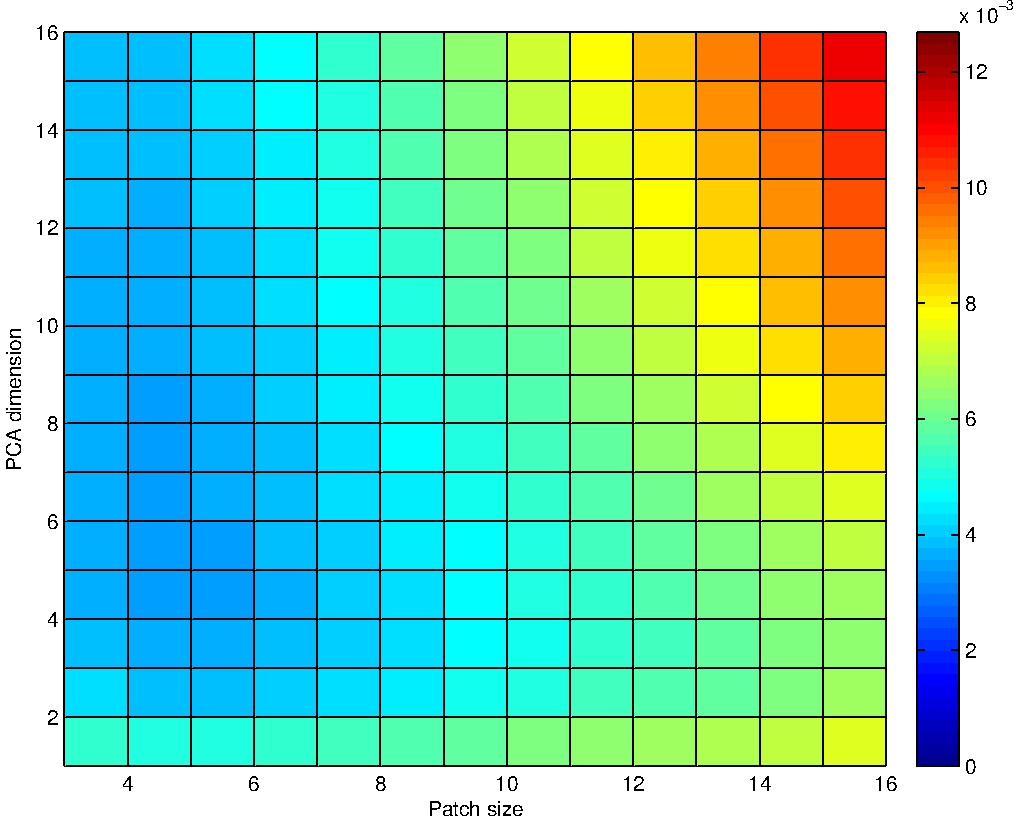
\includegraphics[width=\columnwidth]{training_scaled_avg_4-64-crop}
    \caption{Scaled average of MSE and compression ratio over a range of patch sizes and PCA dimensions.}
    \label{training_scavg}
\end{figure}

It is also important to consider the effect of these parameters on running time. In particular the parameter $k$ has a significant effect on the speed of the K-means subalgorithm, as measured in figure \ref{cpu_k}. Interestingly, the number of iterations to convergence is extremely unpredictable, which may be due to dimension reduction rendering clusters less distinguishable.

\begin{figure}[tbp]
    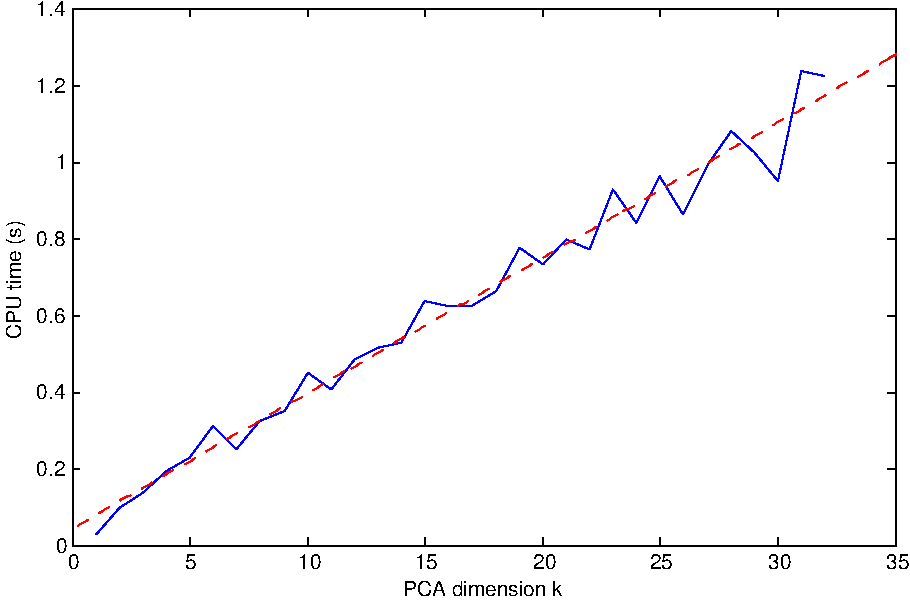
\includegraphics[width=\columnwidth]{cpu_pca-crop}
    \caption{CPU time for K-means clustering against number of retained principal components.}
    \label{cpu_k}
\end{figure}

\subsection{Implementation details}
In addition to the basic algorithm described above, we introduce a couple of practical modifications to improve the runtime and visual quality of the output. Since applying Lloyd's algorithm over $n$ points is time-consuming for large images, we compute the centroids on a random sample of $10\%$ of the data, then assign the remainder of the points according to their distance to these centroids. The impact in terms of accuracy of reconstruction of such a modification is small, but the increase in speed of the clustering step is significant.

One issue in the reconstruction of the original image is that it tends to introduce spurious high-frequency components on the edges of patches. Since it is unlikely that such components were present in the original image, we apply a simple low-pass filter to the pixels on the patch boundaries. This enhances the visual quality of the image and reduces `blockiness'.
\section{Results}
\label{results}
\section{Discussion}
\label{discussion}
\input{summary}




\bibliographystyle{plain}
\bibliography{references}

\end{document}







